\documentclass[12pt]{article}
\title{ Data Mining (CSCI B-565) \\
Assignment No. $3$ \\
Masters in Data Science \\Indiana University\\ Bloomington, IN, USA}
\author {Abhishek Rapelli \\ arapellii@iu.edu}
\date{\today}
\usepackage{fullpage}
\usepackage{amsmath,amssymb}
\usepackage{graphicx} 
\begin{document}
\maketitle
\begin{center}
\textit{All the work herein is solely mine}
\end{center}
\begin{enumerate}
	
\item[1.] (a) The setosa species is red color, the versicolor species is green color and the virginica species is blue color. We can see this from the scatter plots generated by the given R code and the corresponding range of values for each color with respect to Sepal length, width and also from the dataset labels.

\begin{center}
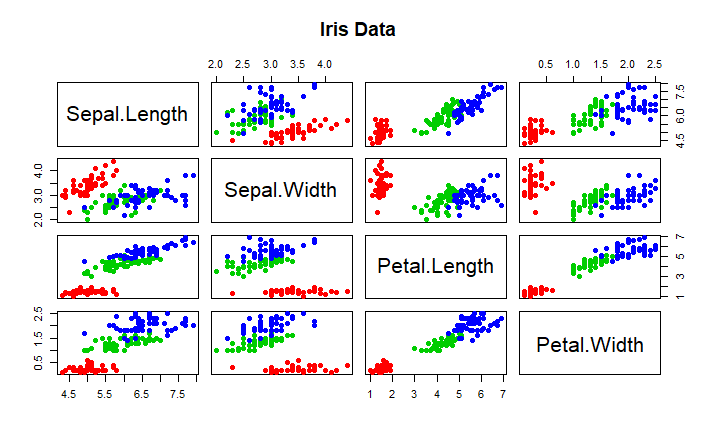
\includegraphics[width=0.5\columnwidth]{DM1} \\	Scatter plots of Iris dataset
\end{center}
(b) The principle components of the given dataset are PC1, PC2, PC3 and PC4. These components  give us a glance of spacial variance of the given dataset and the direction corresponding to highest variance \\
\newpage
(c) From the curve we see that it bends at PC2 and PC3, Hence we will consider PC1, PC2 and PC3 as we have maximum area under the curve. For PC1 we have 0.733 value, but the value increases to 0.959 when we consider PC2 also. Hence we should be considering PC1 and PC2. Using the components with variance >= 1, but only PC1 has the standard deviation of 1.7125. Thus we shall take only PC1. \\

(d) The first two unit eigenvectors are PC1(0.5038236, -0.3023682 , 0.5767881, 0.5674952) and PC2 (-0.45499872 ,-0.88914419 , -0.03378802 , -0.03545628). Unit eigenvectors are the eigen vectors with a magnitude of 1 and they can be obtained by dividing the eigen vector its magnitude. \\

(e) The log transformation is applied generally to reduce the skewness of the data distribution. The Log application is important because the range of the values are compressed, making it simpler and it has very minimal effect on outliers. When we do not perform the log transformation on the given data during the calculation of the principle components, We see not much difference in our curve as there is a slight bend in our curve and the values on the axis change proportionally. \\

\item [2.] 
Entropy of X: \\
$H(\arrowvert X \arrowvert)$ = -(2/20)log(2/20)-(2/20)log(2/20)-(16/20)log(16/20)\\
$H(\arrowvert X \arrowvert) = 0.9219281$\\

Entropy of Y:\\
$H(\arrowvert Y \arrowvert)$ = -(4/20)log(4/20)-(1/20)log(1/20)-(15/20)log(15/20)\\
$H(\arrowvert Y \arrowvert) = 0.9917601$\\

Entropy of Z: \\
$H(\arrowvert Z \arrowvert)$ = -(10/18)log(10/18)-(4/18)log(4/18)-(4/18)log(4/18)\\
$H(\arrowvert Z \arrowvert) = 1.435521$\\

It doesn't make sense to compute the entropy of X, Y; Y, Z and X, Z as these multisets are not equal in cardinality.\\

If we have another multiset W and its entropy is 0, then it will have only one member but he number of elements belonging to the member in the multiset must be >= 1.\\

In case the multiset W has the same entropy as X, then it will be having the same members as X. Different multisets can have the same entropies for different number of elements as the entropy depends only on the ratio of the occurance of the elements in the multiset. One way of considering the number of elements in W is to have a multiset equal to X. \\

The primary difference between multi sets and probability distribution is that we can apply probability distribution on continuous data but this is not possible in multi sets as we have to discretize the data first. Probability distribution gives us the proportion of a value in the dataset but multiset gives us the occurance of the value and we have to calculate the proportion from it. \\
\item [3.] Consider the following data:
\begin{center}
	$\Delta = \{((a,a,a),5),((b,b,a),10),((a,a,b),5),(b,b,a),10)\}$
\end{center}
Lets create a relation instance r that describes ∆: \\
\begin{center}
 \textbf{A1 \qquad A2 \qquad A3 \qquad L} \\
 a \qquad \quad a \qquad \quad a \qquad \enspace 5  \\
 b \qquad \quad b \qquad \quad a \qquad \enspace 10  \\
 a \qquad \quad a \qquad \quad b \qquad \enspace 5  \\
 b \qquad \quad b \qquad \quad a \qquad \enspace 10  \\
 \end{center}
Entropy of the Label (L): \\

 $H(\Delta \arrowvert L \arrowvert) = -(2/4)log(2/4)-(2/4)log(2/4)$ \\
 $H(\Delta \arrowvert L \arrowvert) = 1$ \\
 
 Entropy of the A1 = a : \\
 $H(\Delta \arrowvert A1 =  \arrowvert) = -(2/2)log(2/2)-(0/0)log(0/0)$ \\
 $H(\Delta \arrowvert A1 = a \arrowvert) = 0$ \\
 
 Entropy of the A1 = b : \\
 $H(\Delta \arrowvert A1 = b \arrowvert) = -(2/2)log(2/2)-(0/0)log(0/0)$ \\
 $H(\Delta \arrowvert A1 = b \arrowvert) = 0$ \\ 
 
The information gain (I) after splitting about A1 is: \\
 $I(\Delta \arrowvert A1 \arrowvert) = H(\Delta \arrowvert L \arrowvert)-(2/4)H(\Delta \arrowvert A1 = a \arrowvert)-H(\Delta \arrowvert A1 = b \arrowvert)$ \\
 $I(\Delta \arrowvert A1 \arrowvert) = 1-0-0 = 1$ \\
 
 Entropy for A2 = a : \\
 $H(\Delta \arrowvert A2 = a \arrowvert) = -(2/2)log(2/2)-(0/0)log(0/0)$ \\
 $H(\Delta \arrowvert A1 = a \arrowvert) = 0$ \\
 
 Entropy for A2 = b : \\
 $H(\Delta \arrowvert A2 = b \arrowvert) = -(2/2)log(2/2)-(0/0)log(0/0)$ \\
 $H(\Delta \arrowvert A1 = b \arrowvert) = 0$ \\
 
 The information gain (I) after splitting about A2 is: \\
 $I(\Delta \arrowvert A2 \arrowvert) = H(\Delta \arrowvert L \arrowvert)-(2/4)H(\Delta \arrowvert A2 = a \arrowvert)- (2/4)H(\Delta \arrowvert A2 = b \arrowvert)$ \\
 $I(\Delta \arrowvert A2 \arrowvert) = 1-0-0 = 1$ \\
 
 Entropy of the A3 = a : \\
 $H(\Delta \arrowvert A3 = a \arrowvert) = -(2/3)log(2/3)-(1/3)log(1/3)$ \\
 $H(\Delta \arrowvert A3 = a \arrowvert) = 0.9182958$ \\
 
 Entropy of the A3 = b : \\
 $H(\Delta \arrowvert A3 = 'b' \arrowvert) = -(1/1)log(1/1)-(0/0)log(0/0)$ \\
 $H(\Delta \arrowvert A3 = 'b' \arrowvert) = 0$ \\
 
  The information gain (I) after splitting about A3 is: \\
  $I(\Delta \arrowvert A3 \arrowvert) = H(\Delta \arrowvert L \arrowvert)-(3/4)H(\Delta \arrowvert A3 = 'a' \arrowvert)- (1/4)H(\Delta \arrowvert A3 = 'b' \arrowvert)$ \\
 $I(\Delta \arrowvert A3 \arrowvert) = 1 - 0.6887218 - 0 = 0.3112782$ \\
 
 Rules:
 \begin{center}
 	$A1 = a \rightarrow L = 5$ \\
 	$A1 = b \rightarrow L = 10$ \\
 	$A2 = a \rightarrow L = 5$ \\
 	$A2 = b \rightarrow L = 10$ \\
 	$A3 = b \rightarrow L = 5$ \\
 	$A1 = a \enspace \& \enspace A3 = b \Rightarrow L = 5$ \\
 	$A2 = a \enspace \& \enspace A3 = b \Rightarrow L = 5$ \\
 \end{center}

Attributes A1 and A2 have the highest values of Information Gain (1). Hence we can choose either node for building the decision tree. \\

The label of (a, b, a) depends on the rules we choose, A1 = a, A2 = b and A3 = a \\
\begin{center}
If $A1 = a \Rightarrow L = 5$ \\
If $A2 = b \Rightarrow L = 10$ \\
\end{center}
\item[4.] Inductive bias refers to a set of assumptions made by a learning algorithm in order to perform induction, i.e., to generalize a finite set of training data into a general model. Without a bias of that kind, induction would not be possible, since the observations can normally be generalized in many ways. Treating all these possibilities equally, i.e., without any bias in the sense of preference for specific types of generalization, predictions for new situations could not be made. \\

\item[5.] \textbf{Table:} \\
\begin{center}
\textbf{A1 \qquad A2 \qquad A3 \qquad A4} \\

A  \qquad \quad x \qquad \quad \quad 1 \quad \qquad 4 \\
B  \qquad \quad x \qquad \quad \quad 2 \quad \qquad 3 \\
B  \qquad \quad y \qquad \quad \quad 2 \quad \qquad 3 \\
A  \qquad \quad w \qquad \quad \quad 1 \quad \qquad 2 \\
C  \qquad \quad x \qquad \quad \quad 2 \quad \qquad 1 \\
C  \qquad \quad y \qquad \quad \quad 2 \quad \qquad 1 \\
C  \qquad \quad z \qquad \quad \quad 2 \quad \qquad 1 \\
A  \qquad \quad v \qquad \quad \quad 1 \quad \qquad 1 \\
C  \qquad \quad v \qquad \quad \quad 3 \quad \qquad 3 \\
C  \qquad \quad y \qquad \quad \quad 3 \quad \qquad 3 \\
B  \qquad \quad w \qquad \quad \quad 2 \quad \qquad 1 \\
B  \qquad \quad z \qquad \quad \quad 2 \quad \qquad 1 \\
A  \qquad \quad x \qquad \quad \quad 1 \quad \qquad 4 \\
A  \qquad \quad z \qquad \quad \quad 1 \quad \qquad 4 \\
A  \qquad \quad w \qquad \quad \quad 1 \quad \qquad 4 \\
\end{center}
\begin{itemize}
	\item[(a)] H(A1) = (6/15)log(15/6) + (4/15)log(15/4) + (5/15)log(15/5) = 1.5655 \\
	
	H(A2) = (4/15)log(15/4)+(3/15)log(15/3)+(3/15)log(15/3)+ (3/15)log(15/3)+(2/15)log(15/2) \\
	= 2.289 \\
	
	H(A3) = (6/15)log(15/6)+(7/15)log(15/7)+(2/15)log(15/2) \\
	= 1.43 \\
	\newpage
	
	\item[(b)] Conditional entropy table: \\
\begin{center}	
	\textbf{A1/A3 \qquad 1 \qquad \quad 2 \qquad \quad 3} \\
	
\quad A \qquad \quad 6/15 \quad \quad \quad 0 \qquad \quad \quad 0 \\

\quad B \qquad \quad \quad 0 \quad \quad \quad 4/15 \qquad \quad 0 \\

\quad C \qquad \quad \quad 0 \quad \quad \quad 3/15 \qquad 2/15 \\
\end{center}
H(A3,A1) = (6/15)log(15/6)+(4/15)log(15/4)+(3/15)log(15/3)+(2/15)log(15/2) \\
$\Rightarrow H(A3,A1) = 1.89$ \\

D(A3, A1) = 1.89-1.43 = 0.46 \\
\begin{center}
	
	\textbf{A1/A2 \qquad A \qquad \quad B \qquad \quad C} \\

\quad x \qquad \quad 2/15 \quad \quad 1/15 \qquad \quad 1/15 \\

\quad y \qquad \quad \quad 0 \quad \quad \quad 1/15 \quad \quad \quad 2/15 \\

\quad w \qquad \quad 2/15 \quad \quad 1/15 \qquad \quad \quad 0 \\

\quad x \qquad \quad 1/15 \quad \quad 1/15 \qquad \quad 1/15 \\

\quad x \qquad \quad 2/15 \quad \quad \quad 0 \qquad \quad \quad 1/15 \\
\end{center}

H(A1/A2) = (4/15)((2/15)log(15/2)+(1/15)log(15)) + (3/15)((1/15)log(15)+(2/15)log(15/2)) + (3/15)((2/15)log(15/2)+(1/15)log(15)) + (3/15)((1/15)log(15)+(1/15)log(15)+(1/15)log(15)) + (2/15)((1/15)log(15)+(1/15)log(15)) \\ 

$\Rightarrow H(A1/A2) = 0.727$ \\
\newpage
\begin{center}
\textbf{A1,A2/A3 \qquad \quad 1 \quad \qquad 2 \quad \quad \qquad 3} \\

(A,x)  \qquad \quad \quad \quad 2/15 \quad \qquad \quad 0 \quad \quad \qquad 0 \\
(A,w)  \qquad \quad \quad \quad 2/15 \quad \qquad \quad 0 \quad \quad \qquad 0 \\
(A,v)  \qquad \quad \quad \quad 1/15 \quad \qquad \quad 0 \quad \quad \qquad 0 \\
(A,z)  \qquad \quad \quad \quad 1/15 \quad \qquad \quad 0 \quad \quad \qquad 0 \\
(B,x)  \qquad \quad \quad \quad \quad 0 \quad \qquad \quad 1/15 \quad \qquad 0 \\
(B,y)  \qquad \quad \quad \quad \quad 0 \quad \qquad \quad 1/15 \quad \qquad 0 \\
(B,w)  \qquad \quad \quad \quad \quad 0 \quad \qquad \quad 1/15 \quad \qquad 0 \\
(B,z)  \qquad \quad \quad \quad \quad 0 \quad \qquad \quad 1/15 \quad \qquad 0 \\
(C,x)  \qquad \quad \quad \quad \quad 0 \quad \qquad \quad 1/15 \quad \qquad 0 \\
(C,y)  \qquad \quad \quad \quad \quad 0 \quad \qquad \quad 1/15 \qquad 1/15 \\
(C,z)  \qquad \quad \quad \quad \quad 0 \quad \qquad \quad \quad 0 \quad \qquad 1/15 \\
(C,v)  \qquad \quad \quad \quad \quad 0 \quad \qquad \quad \quad 0 \quad \qquad 1/15 \\
\end{center}

H(A3/A1,A2) = 2*(2/15)*((2/15)log(15/2)) + 9*(1/15)*((1/15)log(15)) + (2/15)*((1/15)log(15) + (1/15)log(15)) \\

$\Rightarrow H(A3/A1,A2) = 0.329$ \\

\item [(c)] I(A1,A2) = H(A1) - H(A1/A2) \\
= 1.5655 - 0.727 \\
$\Rightarrow I(A1,A2) = 0.8385$ \\

\item [(d)] D(A3,A1) = H(A3,A1) - H(A3) \\
= 1.89 - 1.43 \\
$ \Rightarrow D(A3,A1) = 0.46$ \\
	
\end{itemize}


\item[6.] The distance between A and B is least, so if we combine these two clusters we get the following: \\

	Q((A, B), C) = min\{Q(A, C), Q(B, C)\} = min\{4, 8\} = \{4\} \\
	Q((A, B), D) = min\{Q(A, D), Q(B, D)\} =  min\{5, 2\} = \{2\} \\
\newpage	
\qquad \quad \quad \textbf{(A B) \quad C \quad \quad D} \\
    
\textbf{(A B)}   \qquad 0         \\  
     
\textbf{C}     \quad \quad \qquad 4 \qquad \quad 0          \\    
    
\textbf{D}    \quad \quad \qquad 2 \qquad \quad 2 \qquad \quad 0  \\


From the above table we have distance between (A B) and D and also between C and D is least. Merging (A B) with D first, we get the following table:\\


Q(((AB)D), C) = min\{Q((AB), C), Q(D, C)\} = min\{4, 2\} = \{2\} \\


     \qquad \quad \quad \quad \quad \textbf{((A B) D) \quad C} \\

\textbf{((A B) D)}   \qquad 0         \\

\quad \textbf{C}     \quad \quad \qquad \qquad 2 \qquad \qquad 0 \\

Final table: \\

\qquad \qquad \qquad \qquad \textbf{(((A B) D) C)} \\

\textbf{(((A B) D) C} \qquad \qquad \quad 0 \\

\begin{center}
	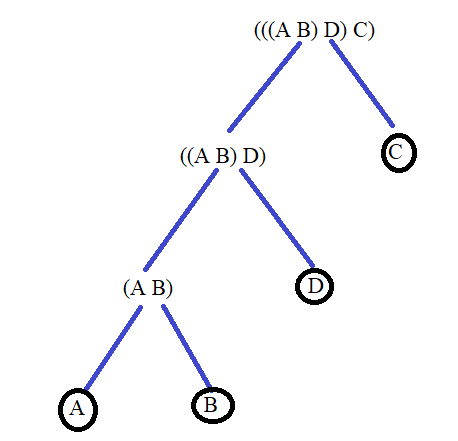
\includegraphics[width=0.5\columnwidth]{Tree} \\
	Tree diagram representation \\
\end{center}


\item[7.] The answer is false because for clustering that has greater than 1000 data points, enumeration of all possible clusters is possible but is not a feasible process. The worst case scenario is when we are having a cluster associated with each data point, which increases the complexity. Similarly, enumeration of all possible clusters increases the runtime exponentially, thus making it not feasible. \\
\item[8.] The answer is false because in agglomerative clustering we perform a linear search for building the proximity matrix and hence the run-time of agglomerative clustering is O($n ^ 2log(n)$), where n is the number of data points. \\

\item[9.] The domain of attributes A1 , A2 and L is \{0, 1\}. Also the information gain for both A1, A2 is same and $H(∆[L]) = k \quad \exists \quad k \textgreater 0.$ \\
The entries that satisfy these conditions are (n \textgreater 1): \\
\begin{center}
\qquad \quad \quad \textbf{A1 \quad A2 \quad L \quad Count} \\

\qquad \qquad 0 \qquad 0 \qquad 0 \qquad n \\

\qquad \qquad 0 \qquad 1 \qquad 1 \qquad n \\

\qquad \qquad 1 \qquad 0 \qquad 1 \qquad n \\

\qquad \qquad 1 \qquad 1 \qquad 0 \qquad n \\
\end{center}

Entropy of Label (L): \\
$H(\arrowvert L \arrowvert)$ = -(2/4)log(2/4)-(2/4)log(2/4) \\
$H(\arrowvert L \arrowvert) = 1$\\

Entropy for A1 = 0 : \\
$H(\Delta \arrowvert A1 = 0 \arrowvert) = -(1/2)log(1/2)-(1/2)log(1/2)$ \\
$H(\Delta \arrowvert A1 = 0 \arrowvert) = 1$ \\

Entropy for A1 = 1 : \\
$H(\Delta \arrowvert A1 = 1 \arrowvert) = -(1/2)log(1/2)-(1/2)log(1/2)$ \\
$H(\Delta \arrowvert A1 = 1 \arrowvert) = 1$ \\

$I(\Delta \arrowvert A1 \arrowvert) = H(\Delta \arrowvert L \arrowvert)-(2/4)H(\Delta \arrowvert A1 = 0 \arrowvert)-H(\Delta \arrowvert A1 = 1 \arrowvert)$ \\
$I(\Delta \arrowvert A1 \arrowvert) = 1-(1/2)-(1/2) = 0$ \\

Entropy for A2 = 0 : \\
$H(\Delta \arrowvert A2 = 0 \arrowvert) = -(1/2)log(1/2)-(1/2)log(1/2)$ \\
$H(\Delta \arrowvert A2 = 0 \arrowvert) = 1$ \\

Entropy for A2 = 1 : \\
$H(\Delta \arrowvert A2 = 0 \arrowvert) = -(1/2)log(1/2)-(1/2)log(1/2)$ \\
$H(\Delta \arrowvert A2 = 0 \arrowvert) = 1$ \\

$I(\Delta \arrowvert A2 \arrowvert) = H(\Delta \arrowvert L \arrowvert)-(2/4)H(\Delta \arrowvert A2 = 0 \arrowvert)- (2/4)H(\Delta \arrowvert A2 = 1 \arrowvert)$ \\
$I(\Delta \arrowvert A2 \arrowvert) = 1-(1/2)-(1/2) = 0$ \\

From the above calculation we can see that, H(∆[L]) = 1 for 1 > 0 thus satisfying the condition. Similarly the information gain for both A1, A2 = 0. \\

\item[10.] \textbf{Noise:} \\

For the corrupt training dataset, a correct decision tree has to address the following two problems: (1) Errors in the training dataset may cause the attributes to become inadequate or may lead to very high complex decision trees. (2) Non-symmetric errors of the values of attributes or class information, which is called "Noise". \\

One solution to this problem is to have the information gain of any tested attribute exceed a threshold value. But this method has a disadvantage, where the tree building process becomes degraded in the noise free case. An alternative method based on the chi-square test for stochastic independence is useful for higher noise levels. The performance of the correct decision tree on corrupted data was found to be inferior to that of an imperfect decision tree formed from corrupted dataset.
\\


\textbf{Unknown Attribute values:} \\

One of the methods for computing the unknown attribute is by placing the most common value, creating a probability distribution, where we can get the most likely value. Another method is to treat all the missing attribute values as a class variable and the class variable as an attribute and then classify based on this. The other method for handling unknown values is to use token values by creating multiple branches at the leaf node level, summation of the value and classifying according to the highest occurance for each class.\\

\item[11.] (a) E(X) = $ \int^{+\infty}_{-\infty} x.p(x) \, dx $ \\
$=$ $ \int^{4}_{-\infty} x.p(x) \, dx + $
$ \int^{+4}_{-4} x.p(x) \, dx +  \int^{+\infty}_{4} x.p(x) \, dx $ \\
$ = 0 +  \int^{+4}_{-4} x.p(x) \, dx + 0 $ \\
$= (1/9)(x^2/2)$ \\
$= (1/9)(4^2/2-(-4)^2/2)$ \\
$= 0$ \\

(b) E(Y) = $ \int^{+\infty}_{-\infty} y.p(y) \, dy $ \\
$=$ $ \int^{4}_{-\infty} y.p(y) \, dy + $ $\int^{+4}_{-4} y.p(y) \, dy +$ $ \int^{+\infty}_{4} y.p(y) \, dy $ \\
$ = 0 +  \int^{+4}_{-4} y.p(y) \, dy + 0 $ \\
$ = 2\int^{+4}_{0} y.p(y) \, dy $ \\
$= 2(1/9)(x^2/2)$ \\
$= 2(1/9)(1^2/2-(0)^2/2)$ \\
$= 16/9$ \\

(c) Mean = E(X) = u = 0 \\
Var(X) = $ \int^{+\infty}_{-\infty} (x-u)^2.p(x) \, dx $ \\
$ = 0 +  \int^{+4}_{-4} (x-u)^2.p(x) \, dx + 0 $ \\
$= (1/9)(4^3-(-4)^3)/3$ \\
$= 128/27$ \\

\item[12.] Probability of 3 appearing = 6/36 \\
The possible outcomes are: \{(3,1), (3,2), (3,4), (3,5), (3,6), (1,3), (2,3), (4,3), (5,3), (6,3), (3,3)\} \\
P('3' on either individual throw of die) $= 6/36 + 6/36 - 1/36 = 11/36$ \\

For the sum being atleast 5, we consider the sum as 5,6,7,8,9,10,11 or 12. This is also same as the sum not equal to 2,3 or 4 . The possible outcomes are \{(1,1), (1,2), (2,1), (2,2), (3,1),(1,3)\} \\

P(the sum less than 5) = 6/36 \\
P(the sum is at least 5) = 1-(6/36) = 30/36 \\

P(A) = P(3 on either individual throw of die) + P(the sum is at least 5) - P(3 on either individual throw of die AND the sum is at least 5) \\
= 11/36 + 30/36 - 9/36 \\
= 32/36 \\
= 8/9 \\

For the difference = 1, we have the following outcomes: {(1,2), (2,1), (2,3), (3,2), (3,4), (4,3), (4,5), (5,4), (5,6), (6,5)}
\\
$\Rightarrow P(B) = 10/36 \\$
If A and B are independent events, then P(A and B) = P(A).P(B) \\
P(A and B) = 8/36 \\
P(A).P(B) = (32/36)(10/36) \\
= (320/1296) \\

Probability of B given A: \\

$P(B \arrowvert A)$ $=$ $P(A $ and $B)/P(B)$ \\
$P(B \arrowvert A) = (8/36)/(32/36) = 1/4$ \\ 

Probability of A given B: \\

$P(A \arrowvert B)$ $=$ $P(A $ and $B)/P(B)$ \\
$P(A \arrowvert B) = (8/36)/(10/36) = 8/10 = 4/5$ \\

\item[13.] (a) PD(X) = $ \int^{+\infty}_{-\infty} f(x) \, dx $ \\
$=$ $ \int^{0}_{-\infty} f(x) \, dx + $
$ \int^{1}_{0} f(x) \, dx +  \int^{+\infty}_{1} f(x) \, dx $ \\
$ = 0 +  \int^{1}_{0} f(x) \, dx + 0 $ \\
$ = \int^{1}_{0} x^ {-1/2}/2  \, dx $ \\
$= (2/2)(x^{1/2}$ \\
$= 1-0$ \\
$= 1$ \\
Since the area below the curve is 1, it is a probability distribution. \\

(b) E(X) = $ \int^{+\infty}_{-\infty} x.f(x) \, dx $ \\
$=$ $ \int^{0}_{-\infty} x.f(x) \, dx + $
$ \int^{1}_{0} x.f(x) \, dx +  \int^{+\infty}_{1} x.f(x) \, dx $ \\
$ = 0 +  \int^{1}_{0} x.f(x) \, dx + 0 $ \\
$ = \int^{1}_{0} x.x^ {-1/2}/2  \, dx $ \\
$ = \int^{1}_{0} x^ {1/2}/2  \, dx $ \\
$ = x^{3/2}/3$ \\
$ = (1^{3/2}-0^{3/2})/3$ \\
$ = 1/3$ \\


(c) Var(x) = $ \int^{+\infty}_{-\infty} (x-u)^2.f(x) \, dx $ \\
$=$ $ \int^{0}_{-\infty} (x-u)^2.f(x) \, dx + $
$ \int^{1}_{0} (x-u)^2.f(x) \, dx +  \int^{+\infty}_{1} (x-u)^2.f(x) \, dx $ \\
$ = 0 +  \int^{1}_{0} (x-u)^2.f(x) \, dx + 0 $ \\
$ = 0 +  \int^{1}_{0} (x-u)^2.x^{-1/2}/2 \, dx + 0 $ \\
$ = 0 +  \int^{1}_{0} (x-1/3)^2.x^{-1/2}/2 \, dx + 0 $ \\
$ = (1/2)\int^{1}_{0} (x^2-2x/3+1/9).x^{-1/2}/2 \, dx $ \\
$ = (1/2)\int^{1}_{0} (x^{3/2}-2x^{1/2}/3+(1/9)x^{-1/2}) \, dx $ \\
$ = (1/2)(2x^{5/2}/5-4x^{3/2}/9+2x^{1/2}/9)$ \\
$ = (1/2)((2/5)1^{5/2}-(4/9)1^{3/2}+(2/9)1^{1/2})$ \\
$ = (1/2)(8/45)$ \\
$ = 4/45$ \\

\item [14.] \textbf{Problem statement:} \\

The given dataset tells us about the sale of individual residential property in Ames, Iowa from 2006 to 2010. The main objective of this project is to predict the selling price of homes \\

\textbf{Observations from the data:} \\

The dataset contains categorical variables with some 'NA' values. This means that the entity that the variable specifies is not present on the property. Replacing all these variable values as ‘NaN’, the missing values in categorical variables are treated by imputing respective mode values. Below is the list of such variables. \\

\begin{center}
	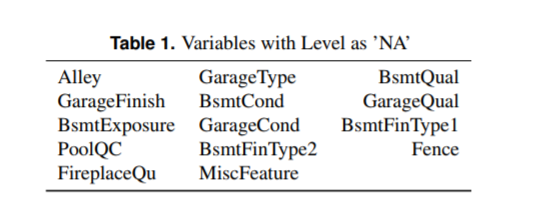
\includegraphics[width=0.5\columnwidth]{H1} \\
\end{center}

\textbf{Treatment of mission values and data cleaning:} \\

Imputing missing values for some of the variables requires domain understanding or knowledge, such as if garage does not exist then there would be zero garage cars, similar with the basement, pool and other property attributes that are missing. \\

\begin{center}
	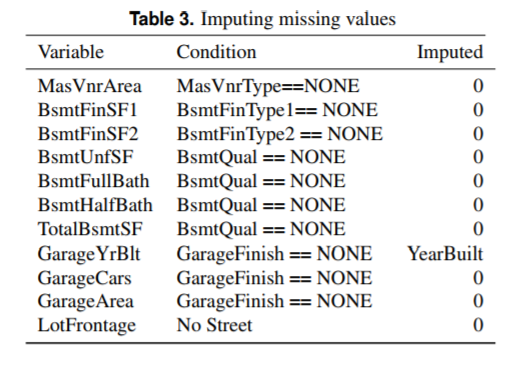
\includegraphics[width=0.5\columnwidth]{H2} \\
\end{center}

\textbf{Data cleaning and implementation code:} \\

\begin{verbatim}
import pandas as pd
import math
import numpy as np
from sklearn import tree

data = pd.read_csv("train,csv")
data = df.fillna(0) #fills NA with 0

Field1 = obj_data.coloums.iloc[:,278]
Field2 = obj_data.coloums.iloc[:,278]
Classifier = tree.DecisionTreeClassifier()
Classifier = Classifier.fit(Field1, Field2) 
\end{verbatim}





\end{enumerate}
\textbf{References}:

\begin{itemize}
	
\item[1.] $https://en.wikipedia.org/wiki/Inductive_bias$ \\
	
\item [2.] $https://books.google.com/books/about/Machine_Learning.html?id=NZP6AQAAQBAJ$ \\
	
\item [3.] $http://www-users.cs.umn.edu/~kumar/dmbook/index.php$ \\

\end{itemize}

\end{document}
